%!TEX spellcheck
%!TEX root = ../bachelor_paper.tex
\documentclass[../bachelor_paper.tex]{subfiles}
\graphicspath{{\subfix{images/}}}
\begin{document}

\chapter{Performance}
    \label{ch:perf}
    
We have observed an expected increase in resource utilization on the \ac{SoC}. datalynx requires additional \acp{LUT}, \acsp{LUTRAM}, \acp{FF}, as well as one additional \ac{BUFG} as seem in table \ref{tab:perf/util/data}. According to the timing analysis performed by Vivado\textsuperscript{\textregistered}, our worst slack interestingly improved from 1.316ns to 1.767ns with the total negative slack being 0ns. Hold slack also slightly improved from 0.054ns to 0.055ns with total negative hold slack again being 0ns. As we have not changed the implementation of the core itself, the changes should be completely transparent to a workload run on the processor, as long as the core frequencies are unchanged. While the critical path for setup slack has not changed in the modified design, the path for hold slack actually has, as can be seen in table \ref{tab:perf/timing/crit}. However, this is occurs within the block diagram wrapper generated by Vivado\textsuperscript{\textregistered} and does not worsen overall hold slack performance significantly.\todo{sind an den limits vom FPGA vll daher?} We thus see this change in critical path as a minor issue if still something to be aware of.

Of note however is the reported increase in power consumption.\todo{nicht ganz so selbstzerstörerisch} As we have enabled the \ac{PS7}, the design requires a lot more power. The unmodified design requires an estimated total of about 0.391W, while the modified version requires about 1.996W, constituting an increase of about 510.486\%. We have not marked power consumption as a priority, as in our opinion an evaluation design for a particular workload is unlikely to have battery longevity or other power related constraints as a point of contention. It is still important to note, as a design incorporating said constraints might look at alternate methods of data logging, given that is what the \ac{PS7} is almost exclusively used for.\\
As seen in figure \ref{fig:perf/power/split}, the share of dynamic power losses increases significantly with the inclusion of the \ac{PS7}. This block alone makes up for about 81\% of power drawn in the modified system. When excluded, power consumption only rises by 76mW compared to the original design. This is still a skewed value however, as other \acp{IP} by Xilinx\textsuperscript{\textregistered}, like the GPIOs and AXI crossbar unit have not been excluded. Including the \ac{PS7} for the modified design leaves us with an estimated junction temperature of 48.0\textdegree C for the modified and 29.5\textdegree C for the unmodified design, resulting in a 37.0\textdegree C and 55.5\textdegree C temperature margin respectively.

\begin{table}
    \centering
    \begin{tabular}{llp{0.73\linewidth}}
    \textbf{Design} & \textbf{Path} \\
    \hline\\[-0.9em]
    \textbf{Unmodified} & From  & \texttt{i\_pulpissimo/soc\_domain\_i/pulp\_soc\_i/jtag\_tap\_top\_i/tap\_top\_i/ td\_o\_reg/C} \\
                        & To    & \texttt{pad\_jtag\_tdo} \\
                        & Setup & 1.32ns \\
    \textbf{Modified}   & From  & \texttt{i\_pulpissimo/soc\_domain\_i/pulp\_soc\_i/jtag\_tap\_top\_i/tap\_top\_i/ td\_o\_reg/C} \\ 
                        & To    & \texttt{pad\_jtag\_tdo} \\
                        & Setup & 1.77ns \\
    \textbf{Unmodified} & From  & \texttt{i\_pulpissimo/soc\_domain\_i/pulp\_soc\_i/soc\_peripherals\_i/ i\_apb\_adv\_timer/u\_apb\_if/r\_timer1\_th\_reg[9]/C} \\
                        & To    & \texttt{i\_pulpissimo/soc\_domain\_i/pulp\_soc\_i/soc\_peripherals\_i/ i\_apb\_adv\_timer/u\_tim1/u\_counter/r\_start\_reg[9]/D} \\
                        & Hold  & 0.05ns \\
    \textbf{Modified}   & From  & \texttt{datalynx\_wrapper\_i/datalynx\_i/axi\_gpio\_4/U0/ ip2bus\_data\_i\_D1\_reg[11]/C} \\
                        & To    & \texttt{datalynx\_wrapper\_i/datalynx\_i/axi\_gpio\_4/U0/AXI\_LITE\_IPIF\_I/ I\_SLAVE\_ATTACHMENT/s\_axi\_rdata\_i\_reg[20]/D} \\
                        & Hold  & 0.05ns \\
    \hline
    \end{tabular}
    \caption{Critical paths for setup and hold slack in unmodified and modified design}
    \label{tab:perf/timing/crit}
\end{table}
\begin{table}
    \centering
    \begin{tabular}{llp{0.15\linewidth}p{0.15\linewidth}p{0.15\linewidth}p{0.15\linewidth}l}
    \textbf{Resource}   & \textbf{Available}    & \textbf{Utilization unmodified} & \textbf{Utilization \% unmodified}  & \textbf{Utilization modified}   & \textbf{Utilization \% modified}    & \textbf{Change}\\
    \hline
    \acs{LUT}           & 53200                 & 43502                     & 81.77\%                       & 46432                     & 87.28\%   & x\\
    \acs{LUTRAM}        & 17400                 & 12                        & 0.07\%                        & 74                        & 0.43\%    & x\\
    \acs{FF}            & 106400                & 22526                     & 21.17\%                       & 28214                     & 26.52\%   & x\\
    \acs{BRAM}          & 140                   & 128                       & 91.43\%                       & 128                       & 91.43\%   & x\\
    \acs{DSP}           & 220                   & 12                        & 5.45\%                        & 12                        & 5.45\%    & x\\
    \acs{IO}            & 200                   & 38                        & 19.00\%                       & 38                        & 19.00\%   & x\\
    \acs{BUFG}          & 32                    & 9                         & 28.13\%                       & 10                        & 31.25\%   & x\\
    \acs{MMCM}          & 4                     & 2                         & 50.00\%                       & 2                         & 50.00\%   & x\\
    \hline
    \end{tabular}
    \caption{Resource utilization unmodified vs. modified}
    \label{tab:perf/util/data}
\end{table}

\begin{figure}
    \centering
    \begin{subfigure}{0.45\textwidth}
        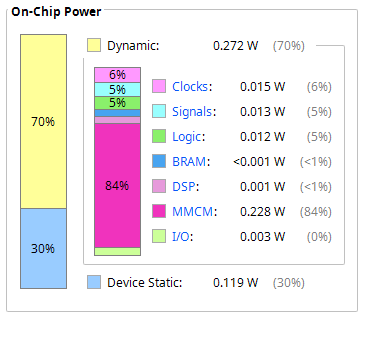
\includegraphics[width=\textwidth]{unmodified_power}
        \caption{Unmodified design}
        \label{fig:perf/power/split/unmod}
    \end{subfigure}
    \hfil
    \begin{subfigure}{0.45\textwidth}
        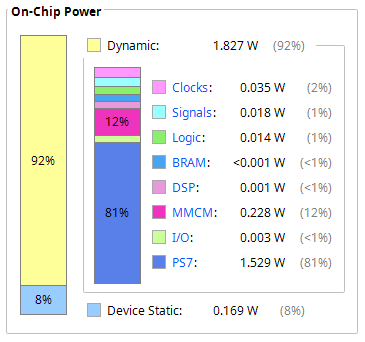
\includegraphics[width=\textwidth]{modified_power}
        \subcaption{Modified design}
        \label{fig:perf/power/split/mod}
    \end{subfigure}
    \caption{Estimated power consumption according to Vivado\textsuperscript{\textregistered}}
    \label{fig:perf/power/split}
\end{figure}

% Render bibliograhy and acronyms if rendered standalone
\isstandalone
\bibliographystyle{IEEEtran}
\bibliography{bibliography}
\subfile{abbreviations.tex}
\fi

\end{document} 
